\documentclass[12pt]{article}
\usepackage{amsfonts}
\usepackage{amssymb}
\usepackage{dsfont}
\usepackage{homework}

\graphicspath{{../figures/}}

\setlength\fboxsep{0.1em} \setlength\fboxrule{0.5pt}
\sethwtitle{ECE661 Homework 8}%
\sethwauthor{Lin Yuan}%
\makehwheader%

\begin{document}
\lstset{language=C++,frame=shadowbox,rulesepcolor=\color{gray},commentstyle=\color{OliveGreen},keywordstyle=\color{blue}\bfseries}
\makehwtitle%

\section{Problem Description}
This homework addresses the problem of object detection using AdaBoost. The problem of object detection is formulated into a binary classification problem, solved with AdaBoost. AdaBoost is considered as one of the best off-the-shelf binary classification algorithm which carries several merits: realtime online testing, consistent generalization error, and high classification rate. On the commonly used datasets like UCI dataset, AdaBoost together with weak classifier Decision Tree is reported to perform very well, along with other competitors such as SVM. After AdaBoost is proposed by \cite{Freund1997}, it has been proven to be convergent in \cite{Friedman1998}, and universally consistent in \cite{Bartlett2007}, which explains why AdaBoost performs well in avoiding the overfitting problem. In this homework, we are going to implement both the original (monolithic) AdaBoost algorithm, together with the Viola-Jones variant -- cascaded AdaBoost algorithm.

\section{Solution}
All major algorithms are explained quite well in the paper of \cite{Viola2004}, but a few keypoints need to be further explained for successful implementation.

\subsection{AdaBoost}
The AdaBoost algorithm is described in Table 1 of \cite{Viola2004}, and is briefly recapitalized here with special directions for implementation.
\begin{itemize}
\item Initialize positive and negative weights. Note here that the weights are different depending on positive and negative sample counts.
\item For t=1 to T, do the following steps. Note that T is the number of weak features you want to select, and this procedure can be done online, by storing the weights from the last iteration t. Which can save computation time in the cascaded version.
\begin{itemize}
\item Normalize the weights to sum to 1.
\item Find best weak classifier using the procedure in Section 3.1 of \cite{Viola2004}. Due to the nature of decision stump, we can have such a efficient implementation.
\item Store the best weak feature and classifier, and the weak classification error, for time t.
\item Update the weights using $w_i^t=w_i^{t-1}\times e^{\frac{\epsilon_t}{1-\epsilon_t}}$.
\end{itemize}
\item Output the final strong classifier. Note that for the calculation of $\alpha_t$,  if the weak classification error $\epsilon_t$ is 0, $\alpha_t$ may be infinite. (Which happens at the case where there is only one negative / positive sample.) In this case, special consideration needs to be taken.
\end{itemize}

\subsection{Cascaded AdaBoost}
The variant cascaded AdaBoost is described in Table 2 of \cite{Viola2004}. Below are a few clarifications for implementation of the cascaded AdaBoost algorithm.

\begin{itemize}
\item $f$ needs to be lower than 0.5, while $d$ can be always kept at 1, however, if one allow $d$ to be a little bit lower than 1, it may help to avoid overfitting, but may be computational costly to find a suitable threshold. In the case of using $d=1$, one can simply keep the threshold for the strong classifier of each stage as the lowest score for positive samples.
\item Each iteration is about training a monolithic AdaBoost classifier on the specific set of positive and negative training samples, until this monolithic classifier, on this specific training set, achieves the false positive rate lower than $f$, and the detection rate higher than $d$.
\item When evaluating for $F_i$ and $D_i$, this evaluation is done using the cascades classifier of all stages until now, on the set of all positive and negative samples.
\item For the inner loop, the training of the monolithic AdaBoost can be done online by storing the previous sample weights.
\item For the outer loop, every time the size of the negative samples is shrank to the false positives of the previous stage, and the positive samples are kept pretty much the same.
\end{itemize}

\subsection{Decision Stump}
Section 3.1 of \cite{Viola2004} details how to find the weak classifier, i.e. a decision stump for a feature.
It can be described as follows:\\
\begin{itemize}
\item Given the vector ${\bf X}_i$ of feature $i$ of all images.
\item Sort ${\bf X}_i$ in decreasing order.
\item Loop from the top to the bottom, and find the total positive weights above the current sample's $i$th feature value (inclusive) and the total positive weights below the current samples's $i$th feature value. Same for the negative weights. Note that in order to keep the information of ``inclusive'', the found threshold $\theta$, should better be stored with double type, and minus a small fraction number such as ``0.1'' to the end.
\item Store the minimum weight error found by splitting the dataset by the threshold $\theta$.
\end{itemize}

\subsection{Finding Haar Features}
The Haar features can be easy to describe, but when actually coding for it, it might take a little bit effort.
Here is the algorithm for finding the vertical and horizontal Haar features.
\begin{itemize}
\item Each horizontal or vertical feature is determined by 6 points.
\item These 6 points are determined by the length and height of the rectangle, and the position of the upper-left corner of the rectangle.
\item Loop through the image pixel positions to fix a upper-left corner.
\item Inner loop, through the feasible length (from pixel position to the border), and an even number
\item Inner inner loop through the feasible height(from pixel position to the border), even or odd number
\item Now depending on the vertical or horizontal configuration, one can determine $x_1,..x_6$.
\end{itemize}

\subsection{Calculating Integral Image}
This is well elaborated in \cite{Viola2004}.


\section{Discussion}
Beyond the above keypoints for successful implementation for AdaBoost, here are a few more tips for debugging and memory allocation.
\begin{itemize}
\item Because haar features are memory-expensive, we need to store them to files first. When storing and reading the haar features, using binary mode can be much faster than storing it using plain text.
\item Debugging AdaBoost is not an easy task for C++. Because usually it might be the case that you won't know where the bug is only after a long time of computation. Always store the cascades stages into files first, and then read in the file directly to debug for the specific stage that the program has bug with.
\item Build with release option and run it on a fast computer.
\item Avoid memory leak by deleting allocated array in time.
\end{itemize}

%\section{Code}\footnote{All source/figures available at:
%\url{http://web.ics.purdue.edu/~yuanl/download/EE661}, require your
%Purdue Career Account Login, only the Professor/TA can access it.}
%\label{src} \sffamily\footnotesize%
%CMakeLists.txt
%\lstinputlisting[language=C++,breaklines=true]{../../code/CMakeLists.txt} %
%hw8.cpp
%\lstinputlisting[language=C++,breaklines=true]{../../code/src/hw8/hw8.cpp} %
%Haarby.h
%\lstinputlisting[language=C++,breaklines=true]{../../code/src/hw8/Haarby.h} %
%Haarby.cpp
%\lstinputlisting[language=C++,breaklines=true]{../../code/src/hw8/Haarby.cpp} %
%AdaBoosby.h
%\lstinputlisting[language=C++,breaklines=true]{../../code/src/hw8/AdaBoosby.h} %
%AdaBoosby.cpp
%\lstinputlisting[language=C++,breaklines=true]{../../code/src/hw8/AdaBoosby.cpp} %
%\rmfamily\normalsize

\section{Results}
The results shown in Fig.\ref{figtest} and Fig.\ref{figtrain} are obtained with a cascaded AdaBoost with $f=0.3$ and $d=1$ for each cascade. The obtained cascade classifier is listed in Table\ref{tabcas}. The first two weak features selected for car detection on the 20 by 40 image. The result of monolithic AdaBoost with 200 features is also shown in Table\ref{tabmono}. Note that the 200 features monolithic AdaBoost can also achieve 0 false positive rate on the training set.

\begin{figure}[!h]
\centering
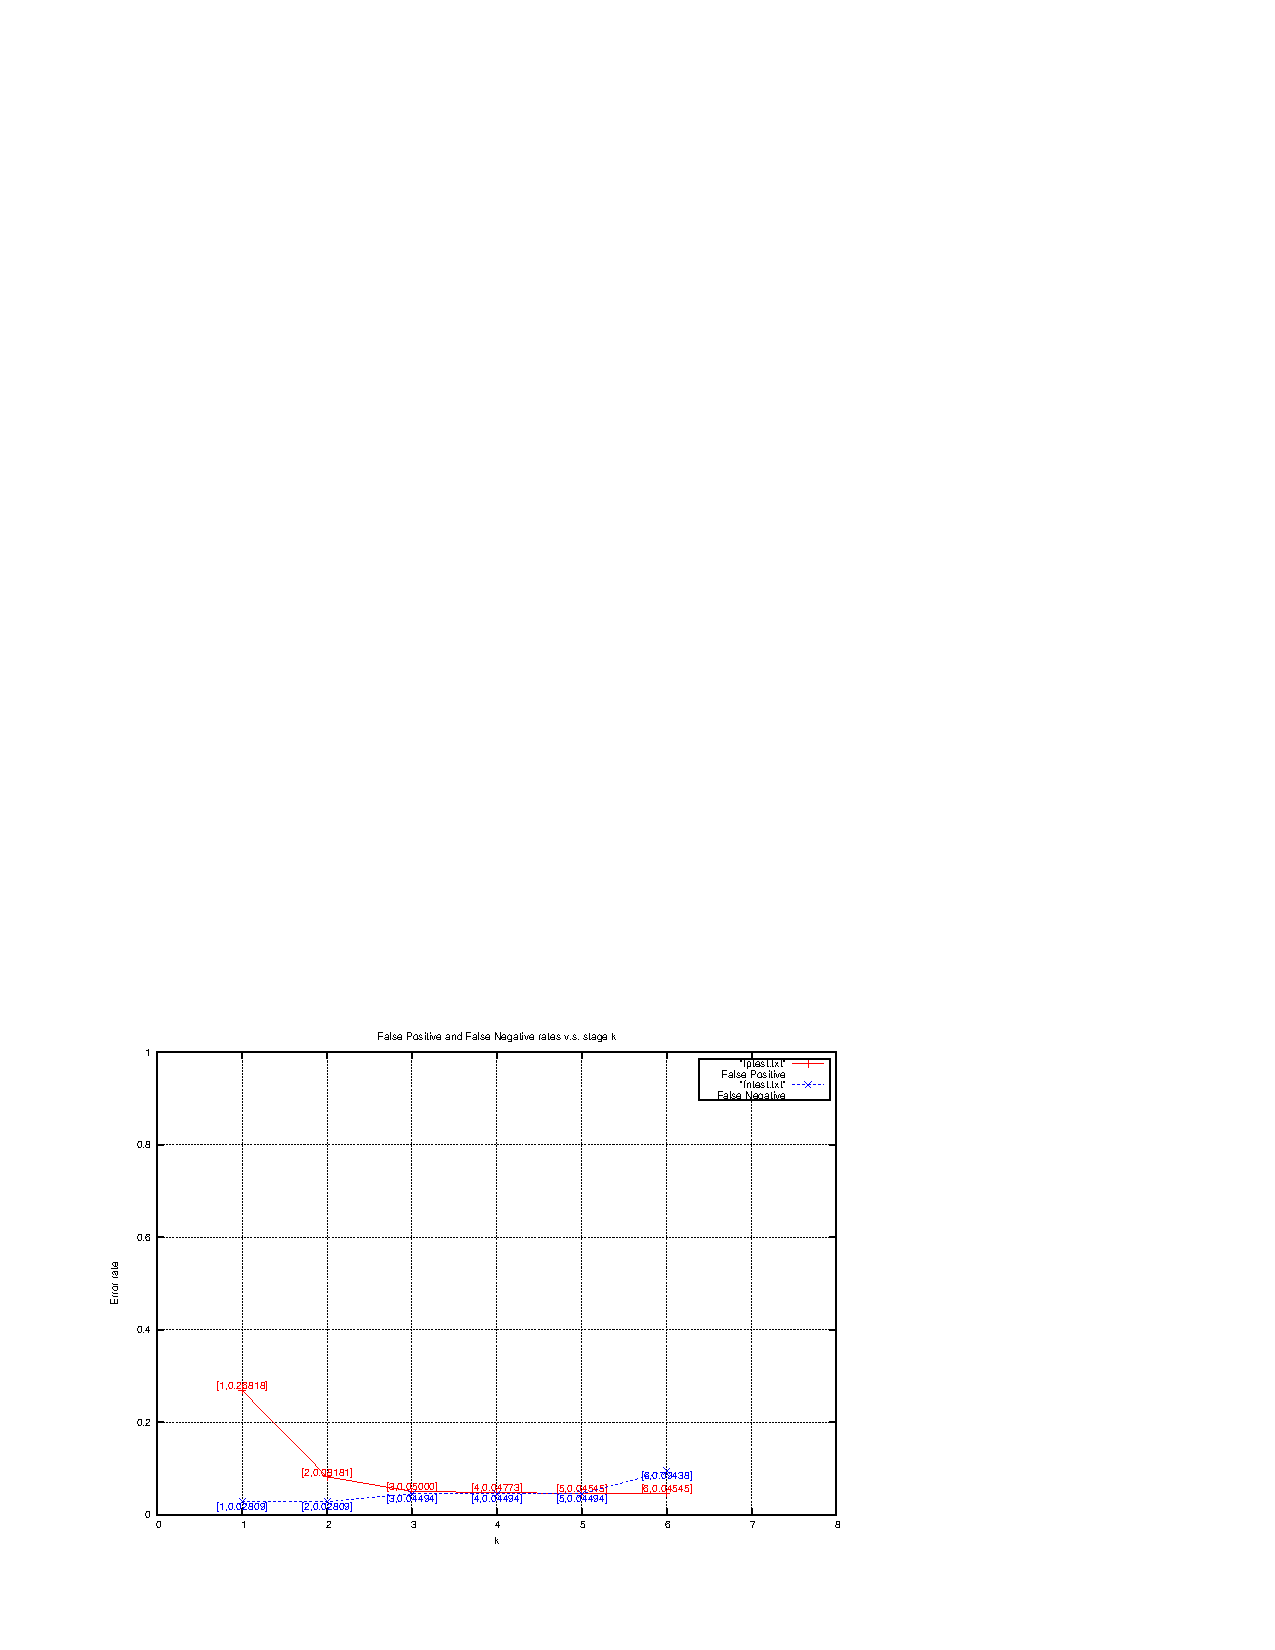
\includegraphics[width=0.85\textwidth]{fpfn_test}
\caption{False positive rate and false negative rate v.s. the number of stages k, for test images \label{figtest}}
\end{figure}
\begin{figure}[!h]
\centering
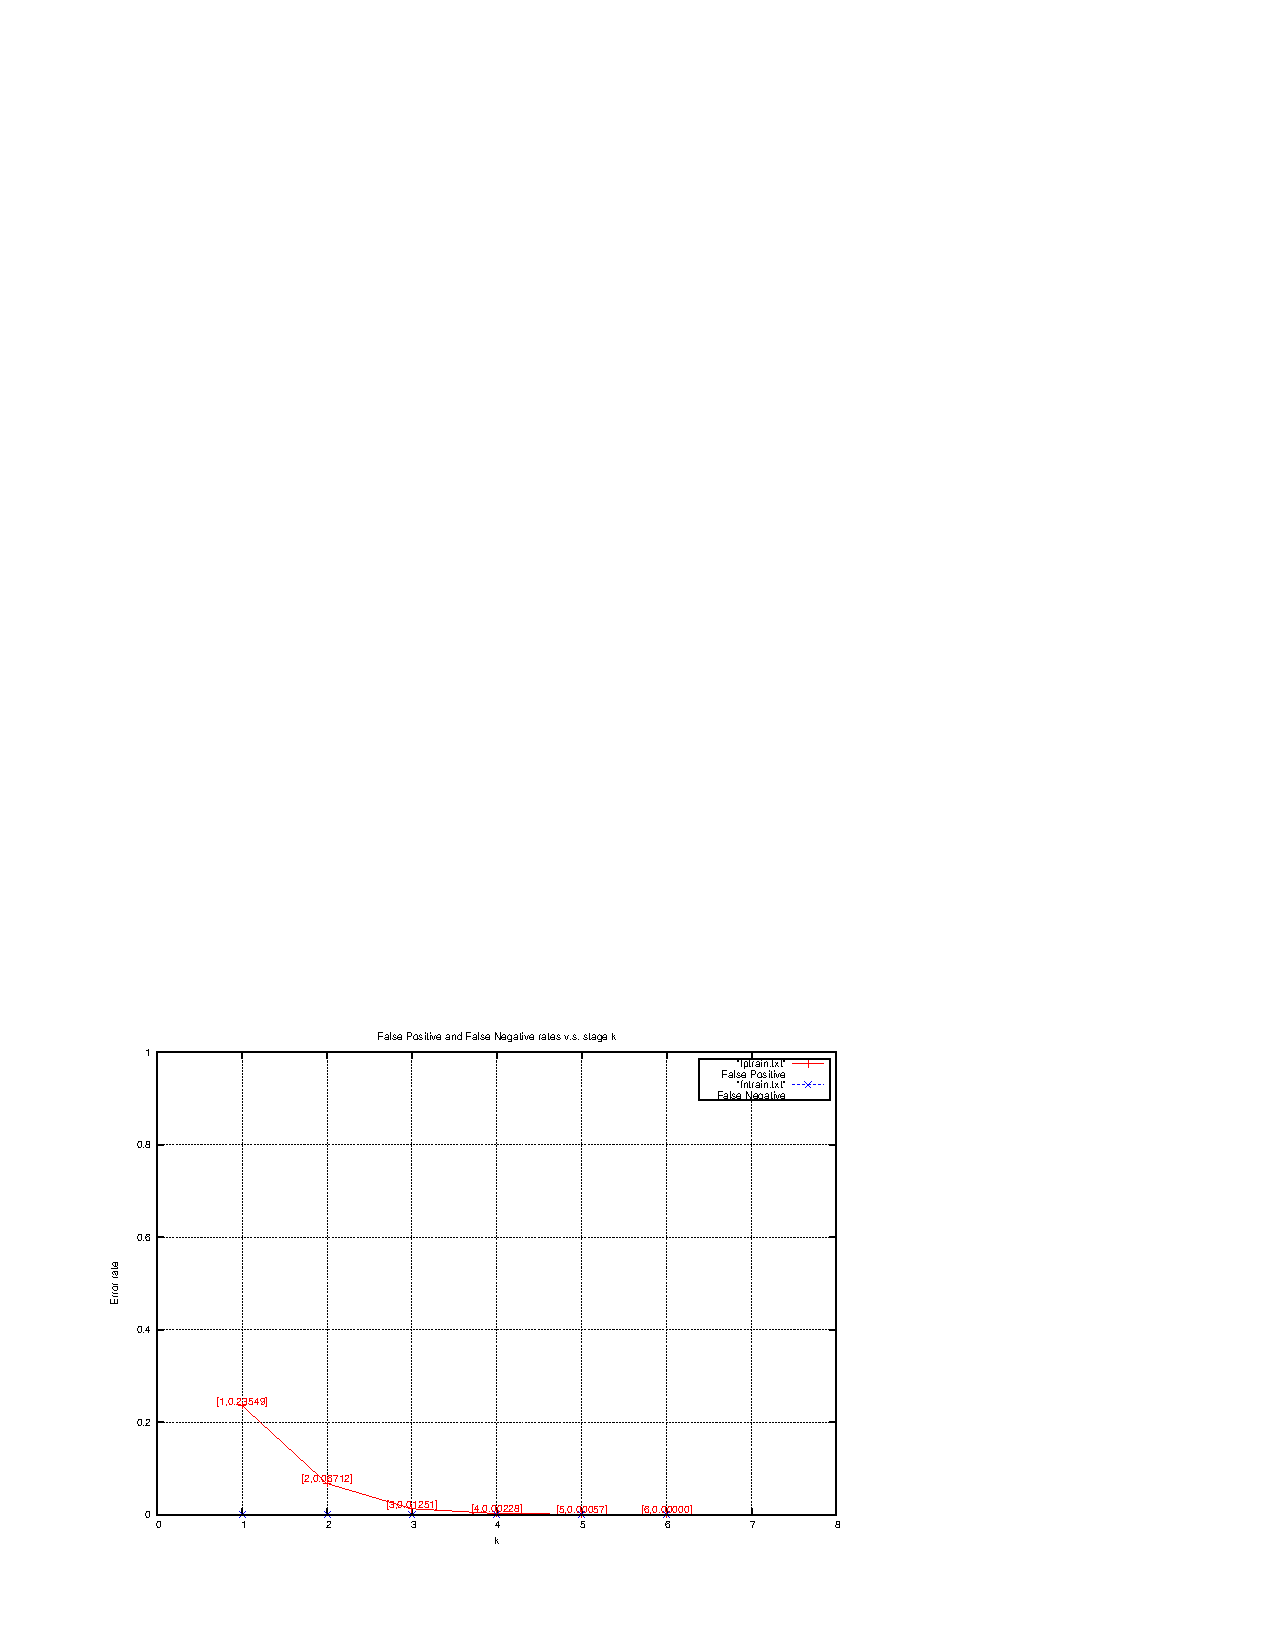
\includegraphics[width=0.85\textwidth]{fpfn_train}
\caption{False positive rate and false negative rate v.s. the number of stages k, for training images\label{figtrain}}
\end{figure}
\begin{table}[!h]
\centering
\begin{tabular}{|c|c|c|c|c|}
\hline
Stage & Haar Index & $\epsilon_t$ & polarity & $\theta$ \\
\hline
1 & 23378 & 0.14997 & 1 & -1101.1 \\
\hline
1 & 72373 & 0.25117 & 1 & -56.1\\
\hline
1 & 123492 & 0.27796 & -1 & 17.9\\
\hline
1 & 158759 & 0.30367 & -1 & 97.9\\
\hline
5 & 2700 & 0.06690 & 1 & 4.9\\
\hline
5 & 120047 & 0.07818 & 1 & 465.9 \\
\hline
5 & 92760 & 0.06835 & -1 & -115.1 \\
\hline
5 & 31300 & 0.08337 & -1 & -87.1\\
\hline
6 & 15519 & 0.0 & 1 & 3732.9 \\
\hline
\end{tabular}
\caption{The cascaded classifier at some stages\label{tabcas}}
\end{table}

\begin{figure}[!h]
\centering
\begin{tikzpicture}[scale=0.3]
\draw (0,0) rectangle +(40,20);
\draw[red] (11,11) rectangle +(17,8);
\draw[green] (0,1) rectangle +(2,14);
\draw[green] (1,1) -- (1,15);
\draw[red] (11,15) -- (28,15);
\end{tikzpicture}
\caption{First two weak features identified for the 20 by 40 car image. Red is feature No. 23378, green is feature No. 72373.\label{carweak}}
\end{figure}

\begin{table}[!h]
\centering
\begin{tabular}{|c|c|c|}
\hline
 & False positive & False negative\\
\hline
Monolithic(200 features) & 0.011 & 0.073 \\
\hline
Cascaded(6 stages) & 0.045 & 0.056\\
\hline
\end{tabular}
\caption{Comparison of monolithic and cascaded AdaBoost applied on the test dataset\label{tabmono}}
\end{table}
\nocite{*}
\bibliographystyle{IEEEtran}
\bibliography{ref}
\end{document}
